% Chapter Template

\chapter{Data Analysis} % Main chapter title

\label{chapter:data} 

%----------------------------------------------------------------------------------------

%----------------------------------------------------------------------------------------

In Chapter \ref{chapter:instrumentation} was described how an ion's $m$, $mpq$ and $v$ can be determined from the PHA data. In this chapter we want to go one step further and obtain the three-dimensional velocity $\vec{v}$ from $v$. \\
For this it is necessary to combine the PHA data with position and orientation information of the Ulysses spacecraft.
Two different coordinate systems are utilized for that. They will be introduced in a first step.


\section{Coordinate Systems}
\label{sec:cs}
In the following analysis the SWICS PHA data will be connected to the position and orientation of the Ulysses spacecraft. For this two different coordinate systems are utilized.

%
\subsection{Heliographic Coordinate System}
Trajectory data from the \citet{ulysses-data-archive} is used in this work to describe Ulysses' orbit. In this data set, Ulysses' position is given in daily intervals and based on different coordinate systems, including the heliographic coordinate system in the B1950.0 epoch.\\
The heliographic (HG) coordinate system is a Cartesian Sun-centered system with the Sun's equatorial plane as a reference plane. Its x-axis is directed along the line of ascending node, which is the intersection line of the ecliptic and the solar equatorial plane. While the latter has an inclination of $i_\odot = 7.25 ^\circ$ against the ecliptic \citep{fraenz_harper} the line of ascending node is at an ecliptic longitude of $\Omega_\odot \approx 75^\circ$ relative to the First Point of Aries in 1950 \citep{nasa-earth-coord}. The z-axis of the HG coordinate system is directed along the Sun's spin axis (northward) and the y-axis completes the right-handed system. \\
In HG spherical coordinates the longitude $\varphi_{\mathrm{HG}}$ is defined to be $0^\circ$ for directions along the x-axis and increases towards the y-axis. The latitude $\vartheta_{\mathrm{HG}}$ is $0^\circ$ for directions within the solar equatorial plane and $+90^\circ$ for northward directions.\\ 
However, when working with the Ulysses trajectory data it was found that these data were given in spherical coordinates for which $\varphi_{HG} = 0^\circ$ was towards $-105 ^\circ$ ecliptic longitude relative to the First Point of Aries. This means that the Ulysses trajectory coordinate system is shifted $180^\circ$ around the solar spin axis against the classical definition (s.a.).\\
In Fig.~\ref{fig:traj} Ulysses' spherical HG coordinates as well as its distance from the Sun are given over the time of the mission.
%
\begin{figure}[h]
	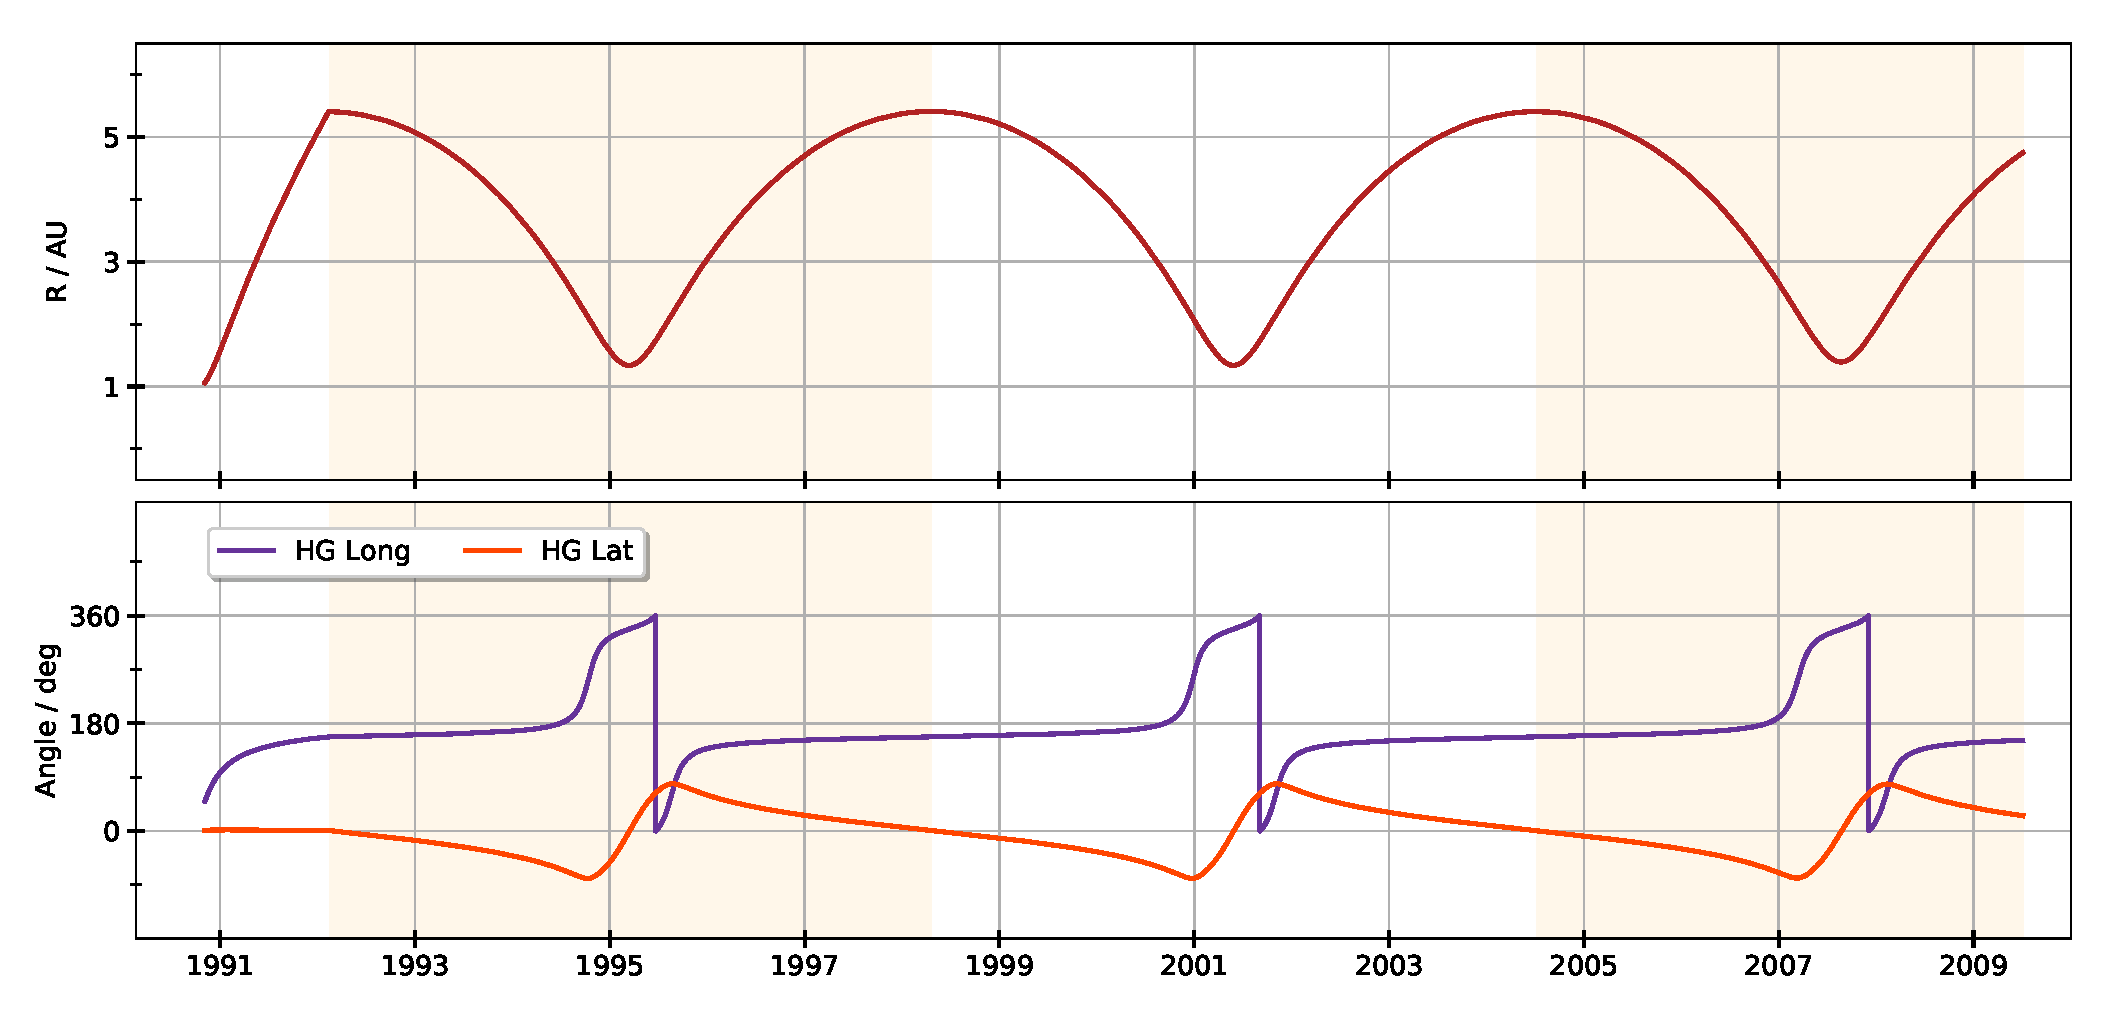
\includegraphics[width=1\textwidth]{Figures/HG_coord.pdf}
	\centering
	\caption{Ulysses trajectory data from November 1990 to June 2009 based on the data from the \citet{ulysses-data-archive}. Color shaded are the three orbits of the mission. \textbf{Upper panel:} Shown is Ulysses' radial distance R from the Sun. Perihelion and aphelion of the spacecraft's elliptical orbit can clearly be seen as the nearest/farthest distance that is $1.3\,\mathrm{AU}$ and $5.4\,\mathrm{AU}$. Over the duration of the mission Ulysses passes each of these points every 6.2 years and three times in total. \textbf{Lower panel:} Shown are Ulysses' HG longitude and latitude. Note that the longitude is shifted by $180^\circ$ with respect to the classical definition (s. text for details). A clear periodicity over Ulysses' three orbits can be seen. Maximum and minimum latitude are $\sim \pm 80^\circ$. These points are highest above the poles of the Sun and are reached a few weeks before and after Ulysses' pass through the perihelion.}
	\label{fig:traj}
\end{figure}

\subsection{Radial Tangential Normal Coordinate System}
Ulysses' orbit has been described in the HG coordinate system, which is a coordinate system that is fixed with respect to the Sun. For describing positions and velocities in the frame of the spacecraft we need a coordinate system that moves with the spacecraft.
\\
When dealing with Ulysses' trajectory data it is useful to work with Radial Tangential Normal (RTN) coordinates. The RTN coordinate system is defined relative to a moving object in the heliosphere, in this case Ulysses, and is centered at the Sun. A graphical representation of the system is given in Fig.~\ref{fig:rtn}. The unit vectors are $\vec{R}$, $\vec{T}$ and $\vec{N}$, where $\vec{R}$ points radially outward from the Sun to the current position of the spacecraft. $\vec{T}$ is defined as the normalized cross product of the Sun's angular velocity, $\vec{\omega}$, and $\vec{R}$. $\vec{N}$ completes the right-handed Cartesian coordinate system. Consequently, the RTN system is not defined for a spacecraft's position right above one of the Sun's poles as the cross product $\vec{\omega} \mathrm{x} \vec{R}$ is zero here. Nevertheless we do not have to worry about this fact as Ulysses did not cross the poles directly.
%
%
\begin{figure}[h]
	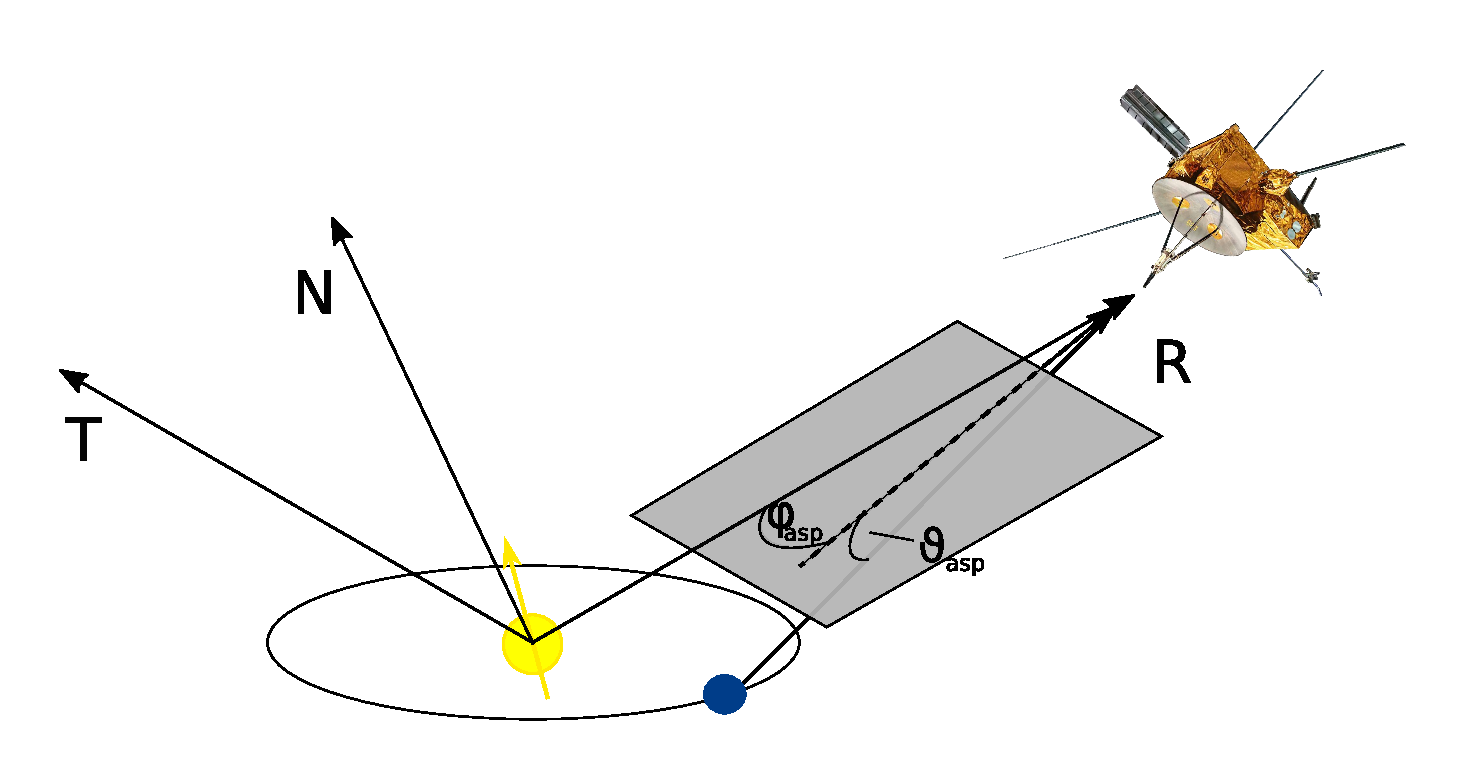
\includegraphics[width=1\textwidth]{Figures/drawing_RTN.pdf}
	\centering
	\caption{Graphical representation of the RTN coordinate system (not to scale). Shown are the Sun (yellow), the Earth (blue) and the Ulysses spacecraft at a non-specific position on its orbit. $\vec{R}$ is defined as the unit vector along the Sun--Earth line, $\vec{T}$ as the normalized cross product $\vec{\omega} \mathrm{x} \vec{R}$ with $\vec{\omega}$ being the angular velocity of the Sun (yellow vector). $\vec{N}$ completes the right-handed Cartesian system. Also shown is the definition of the aspect angle components $\varphi_{\mathrm{asp}}$ and $\vartheta_{\mathrm{asp}}$ as they are used in this work. The grey plane depicts the $\vec{R}$--$\vec{T}$ plane. $0 ^\circ < \varphi_{\mathrm{asp}} < 90^\circ$ and $-90 ^\circ < \vartheta_{\mathrm{asp}} < 0^\circ$ in the shown situation. The Ulysses Image is taken from \cite{esa_orbit} and modified.}
	\label{fig:rtn}
\end{figure}
%
%
%
\section{The Detector Model}
As described in Chapter \ref{chapter:instrumentation}, SWICS can distinguish between three different inflow directions of ions by the threefold division of solid-state detectors. A second directional information can be obtained by the rotation of SWICS being fixedly mounted on the spinning spacecraft as one spin of Ulysses is divided into eight sectors. These two additional measurements allow us to derive a three-dimensional velocity $\vec{v}$ of incident ions.\\
With each Triple Coincidence PHA word we receive information of which of the three solid-state detectors has been hit and in which of the eight sectors the measurement took place. However, a sector-detector information alone is not sufficient to determine the ion's three-dimensional velocity. Its meaning is highly dependent on SWICS' orientation and the eigen-velocity of the spacecraft. Additionally, SWICS' collimator is characterized by an intricate geometry, making an analytical solution of the problem difficult. Instead, we choose to use a virtual detector as a numerical approach. The initial idea of modelling the SWICS detector comes from Dr. Lars Berger who constructed a similar model for ACE SWICS. This work focusses on establishing the model for Ulysses SWICS.

%Was macht das Modell? -- Ich will das FoV zu jedem Zeitpunkt bestimmen. Ich nehme dafür einzelne Messpunkte auf der originalen Geometrie. Dann gebe ich noch ins Modell, wie das gerade ausgerichtet ist.\\
%Berechnet anhand des AA, wohin Sun trigger schaut, wenn getriggert wird und rotiert coll. an entsprechende Position für Sek 0. Ordnet entsorechend andere Sektoren an.
%Simuliert FoV durch Punkteraster \\


%
%
%
\begin{figure}
	\centering
	\begin{subfigure}{.5\textwidth}
		\centering
		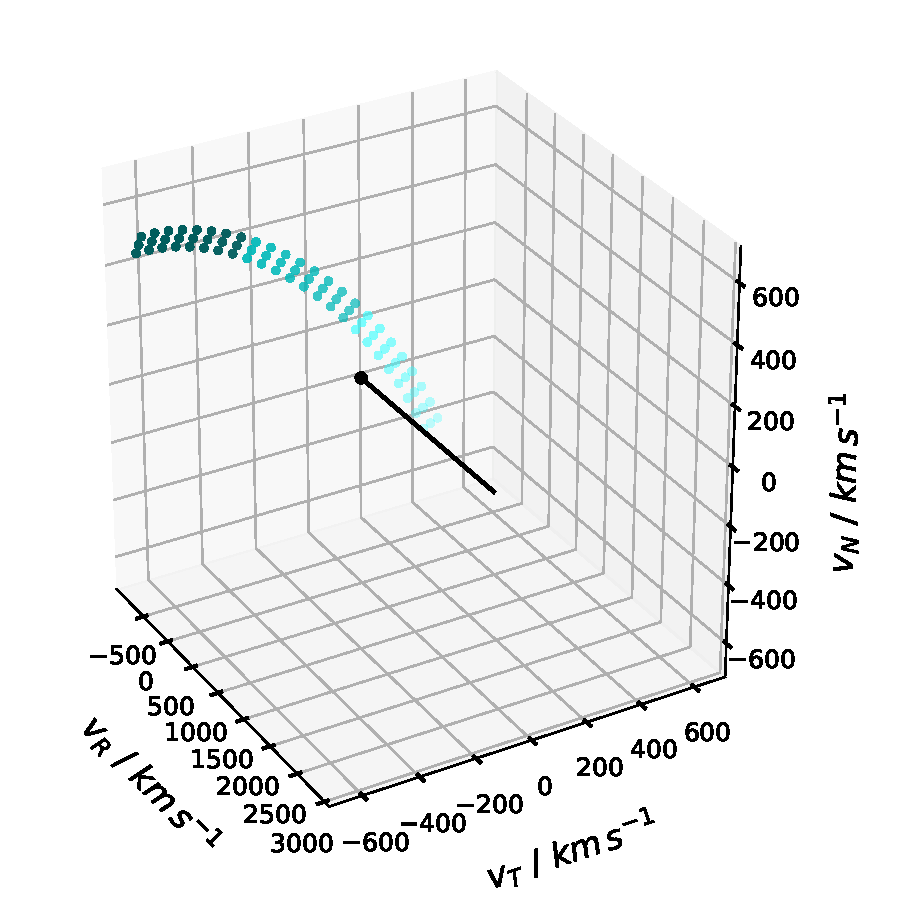
\includegraphics[width=1\linewidth]{Figures/col_single_new.pdf}
	\end{subfigure}%
	\begin{subfigure}{.5\textwidth}
		\centering
		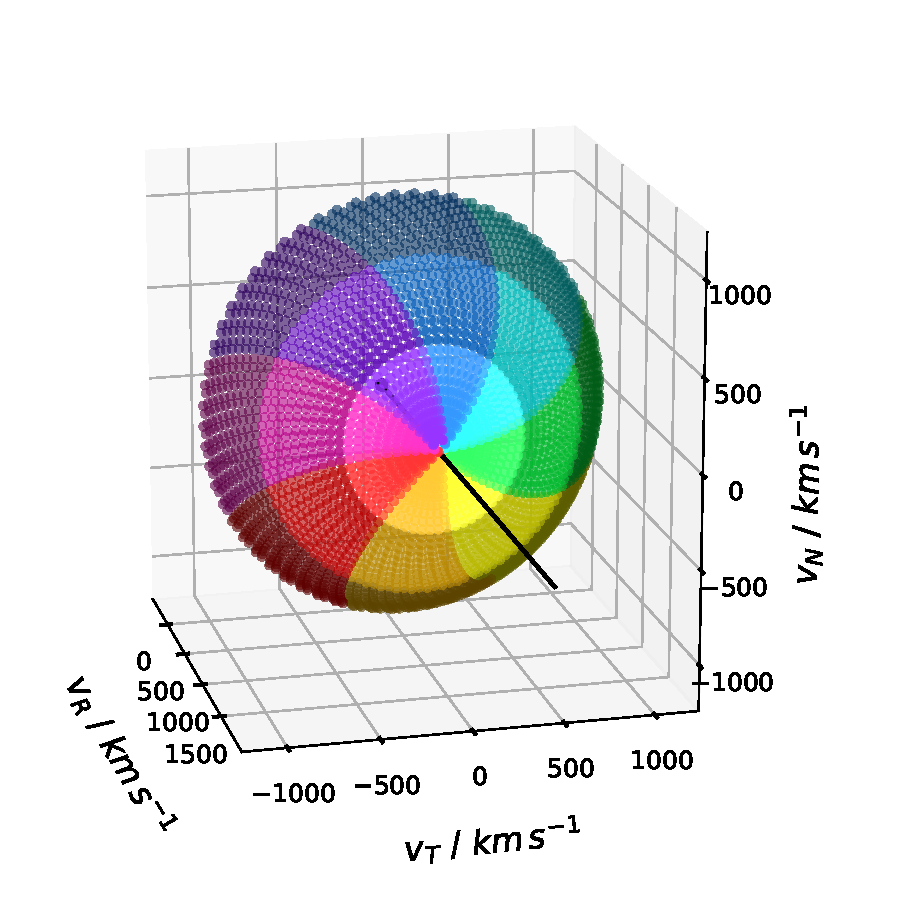
\includegraphics[width=1\linewidth]{Figures/col_vspace_normal.pdf}
	\end{subfigure}
	\caption{Velocity acceptance volume for ESA step 10 ($v \sim 1200\,\mathrm{km\,s^{-1}}$)  For a fixed instrument (\textbf{left Panel}) and integrated over one spin that is divided into eight sectors (\textbf{right Panel}). The differently shaded areas indicate the acceptances of the three solid-state detectors. The black line shows the radial direction, i.e. velocities towards the Sun.}
	\label{fig:coll_FoV}
\end{figure}
%
\begin{figure}[h]
	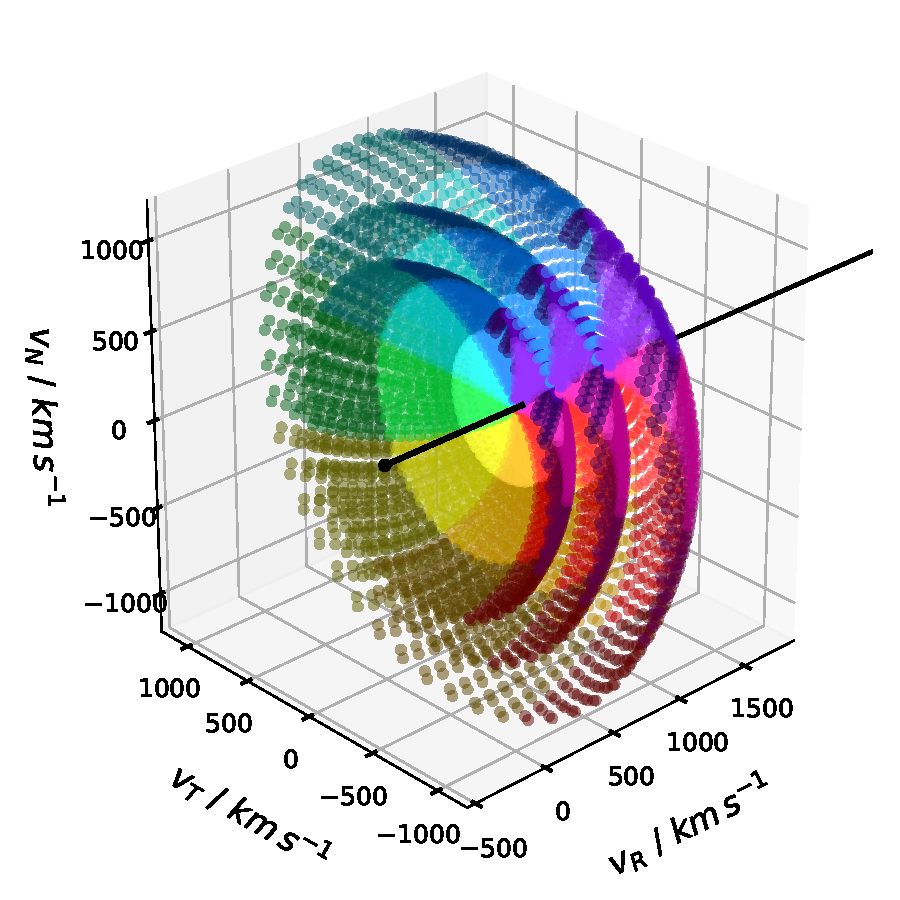
\includegraphics[width=0.5\textwidth]{Figures/col_shells.pdf}
	\centering
	\caption{Velocity acceptance volume for three ESA steps 4, 10 and 17. Acceptance velocities on each shell have the same velocity $v_i$, i.e. the same distance to $v = 0\,\mathrm{km\,s^{-1}}$ (black dot) in this plot. $v_i$ corresponds to the respective ESA step}
	\label{fig:coll_shells}
\end{figure}
%
%
%
\subsection{Construction} 
\label{subsec:construction}
\begin{figure}[h]
	%\includegraphics[width=0.5\textwidth]{Figures/FOTO_VOM_3D_PRINT.pdf}
	\includegraphics[width=0.5\textwidth]{Figures/foranne.png}
	\centering
	\caption{3D printed model of SWICS' entrance system that was made from the original CAD files. Its geometry can be described by a cut of $90\,^\circ$ longitude from a sphere at $56 ^\circ$ polar latitude. The resulting piece is not flat but curved and has a height of $\sim 5\,\mathrm{cm}$. This geometry leads to two deflection plates that are curved but have a constant distance of $\sim 3.7\,\mathrm{cm}$ over a relatively large area which is necessary to provide a constant voltage for the energy-per-charge filtering action (s. Sec.~\ref{sec:EpQ}). The resulting opening angles of the collimator are $69^\circ$ in width and $4^\circ$ in height. The x-axis depicts the direction of Ulysses' spin axis, the three vectors are normals on the opening of the detector. Particles with velocity vectors antiparallel to those vectors can enter.}
	\label{fig:3dcol}
\end{figure}
For reconstructing the velocity space that is observed by SWICS we need to know the possible directions of incident particles that can enter the instrument. These directions are limited by the instrument's entrance system.
\\
The original geometry of the SWICS entrance system was read out from a CAD model. To illustrate the intricate geometry, a photo of a 3D printed model of the entrance system is shown in Fig.~\ref{fig:3dcol}.\\
The instrument is mounted with one of the collimator's narrow side edges parallel to Ulysses' spin axis. When we define this edge to be lying on the x-axis of a three-dimensional Cartesian coordinate system, the collimator geometry can be reconstructed by revolving this edge for $90^\circ$ around a straight line that lies in the xy-plane with an angle of $56^\circ$ relative to the x-axis.  These $90^\circ$ are divided into three parts, each of which is reserved as the opening angle for one of the three detector elements that are described in Sec.~\ref{sec:swics}. \\ \\
The detector's field of view is the solid angle over which the detector is sensitive to incoming particles.
It can be represented by a set of outward directed normal vectors on the opening plane of the detector (exemplary vectors $\mathrm{\mathbf{f_1}}$, $\mathrm{\mathbf{f_2}}$ and $\mathrm{\mathbf{f_3}}$ in Fig.~\ref{fig:3dcol}). In our model, we have a variable number $n_\mathrm{d}$ of these equidistant vectors which we can divide along the width and the height of the detector opening. The real continuous field of view is modelled better with an increasing number of normal vectors that cover the opening. \\
Each of these normalized vectors $\mathrm{\mathbf{f_i}}$ has a unique direction $\mathrm{\mathbf{f_i} = \begin{bmatrix}f_{x,i}\,f_{y,i}\,f_{z,i}\end{bmatrix}}'$ in position space.
\\
With a spin of the Ulysses spacecraft the fixedly mounted SWICS instrument is revolved around the spacecraft spin axis. One revolution of SWICS is divided up into eight sectors of approximately equal duration, each covering $45^\circ$ (s. Sec.~\ref{sec_dataprod}). As the spacecraft is spinning continuously, also the field of view changes its rotation angle continuously. For our virtual detector we model this by rotating the field of view gradually over $n_\mathrm{sec}$ steps through every sector.\\
The integrated field of view over one spin then comprises $n_\mathrm{FoV} = n_\mathrm{d} \cdot n_\mathrm{sec} \cdot 8$ single vectors $\mathrm{\mathbf{f_i}}$ which are directed symmetrically around the spin axis.
%
%
%
\subsubsection{From Field of View to Velocity Space}
The detector's velocity acceptance can be calculated by combining the directional information from the field of view with the value of absolute velocity from the current ESA step. 
\\
Limited by the collimator, a particle can only enter the detector when its absolute velocity is within the acceptance of the current ESA step and when its velocity vector is antiparallel to the detector's field of view. For a given acceptance velocity $v_i$, each field of view vector $\mathrm{\mathbf{f_i} = \begin{bmatrix}f_{x,i}\,f_{y,i}\,f_{z,i}\end{bmatrix}}'$ can be associated with an acceptance velocity vector
\begin{align}
\mathbf{v_i} = \begin{bmatrix}v_{R,i}\\v_{T,i}\\v_{N,i}\end{bmatrix} = - \begin{bmatrix}f_{x,i}\\f_{y,i}\\f_{z,i}\end{bmatrix} \cdot v_i.
\label{eq:fov}
\end{align}
The resulting acceptance of the fixed instrument for $n_d = 72$ and $v \sim 1200\,\mathrm{km\,s^{-1}}$ is shown in Fig.~\ref{fig:coll_FoV}, left panel. \\
With consideration of the integrated field of view over one spacecraft spin the acceptance velocity for a distinct velocity $v_i$ consists of the combination of $n_\mathrm{FoV}$ discrete velocities which form a dome with radius $v_i$ in velocity space, s. Fig.~\ref{fig:coll_FoV}, right panel, for $v \sim 1200\,\mathrm{km\,s^{-1}}$)
\\ \\
The central velocity for an ion of charge $q$ and mass $m$ at an ESA step with energy-per-charge $EpQ$ (in $keV/e$) is
\begin{align*}
\frac{v_c}{km \, s^{-1}} = \sqrt{\frac{2 \cdot EpQ \cdot 1.602\cdot10^{-19}\cdot |q|}{m \cdot 1.661 \cdot 10^{-27}} }
\end{align*}
with $m = 4\,\mathrm{u}$ and $|q| = 1\,\mathrm{e}$ for $\mathrm{He^{+}}$.
\\
Different absolute velocities $v$ appear as distinct shells of radius $v$ in velocity space.
To get an idea of this, an example with three of those (ESA steps 4 ($v \sim 1480 \,\mathrm{km\,s^{-1}}$), 10 ($v \sim 1190 \,\mathrm{km\,s^{-1}}$) and 17 ($v \sim 930 \,\mathrm{km\,s^{-1}}$)) shells is shown in Fig.~\ref{fig:coll_shells}.\\
To represent the uncertainty in the energy-per-charge measurement, we take into account the relative uncertainty $\Delta \frac{E}{q}/\frac{E}{q} = \pm 2.5\%$ \citep{gloeckler_1992} and translate it into an uncertainty $\Delta v / v = \frac{1}{2} \left( \Delta \frac{E}{q}/\frac{E}{q}\right) = \pm 1.25\%$ in accepted velocity. For every ESA step we can now choose a number of $n_{epq}$ single velocities that are distributed evenly in the interval $\left[ v_c - \Delta v / v, v_c + \Delta v / v \right]$. %The total number of accepted absolute velocities $v$ is then $64 \cdot n_{epq}$.
\\
By combining all $64 \cdot n_{epq}$ shells we obtain a dense three-dimensional pattern of accepted velocities that simulate the real continuous velocity acceptance volume of the spinning detector.
\\ \\
When we measure a PHA word with a distinct sector, detector and ESA information, we can now determine a set of three-dimensional velocities with which the particle could have entered the instrument. Of course, the resolution is limited as sector and detector areas are finite and because of the uncertainty $\Delta \frac{E}{q}/\frac{E}{q}$. By spreading the count over the entirety of ($n_i = n_{epq}\cdot n_{sec} \cdot n_{d} \cdot \frac{1}{3}$) absolute velocity acceptances in the volume of the sector-detector-ESA combination, we assign a set of equally likely possible velocities to the count.
%
%
%
\subsection{Ulysses' Eigen-velocity}
For the considerations in the previous section we assumed a detector on a spacecraft that is fixed in space. Obviously this is not the case for the Ulysses spacecraft,  which moves on its elliptical orbit around the Sun. When considering a velocity measurement from a moving spacecraft, the actual velocity in an external frame of reference is determined as an addition of the measured velocity and the spacecraft's eigen-velocity.\\
For determining the spacecraft's velocity we make use of the daily trajectory data from Sec.~\ref{sec:cs}. For every point in time $t_i$ we calculate the spacecraft's instantaneous velocity $v_{SC,i}$ by forming the differential quotient 
\begin{align*}
v_{SC,i} = \frac{ \begin{bmatrix}R_{i+1}\\T_{i+1}\\N_{i+1}\end{bmatrix}_i  - \begin{bmatrix}R_{i}\\T_{i}\\N_{i}\end{bmatrix}_i} {t_{i+1} - t_i}
\end{align*}
with $t_{i+1}$ being the time of the next trajectory data given, which is normally $t_i + 1\,\mathrm{d}$. Note that the spacecraft's position at $t_{i+1}$ has to be considered in the RTN coordinate system that relates to the spacecraft's position at $t_i$. The resulting velocities in RTN coordinates are shown in Fig.~\ref{fig:eigenv} and range between $-20\,\mathrm{km\,s^{-1}}$ and $35\,\mathrm{km\,s^{-1}}$.
\\
To correct the measured velocities for the spacecraft's eigen-velocity, we add the resulting eigen-velocity components to the velocity acceptance. Thus, for every instant in time the shells in Fig.~\ref{fig:coll_shells} are shifted a bit in velocity space based on the respective eigen-velocity.

\begin{figure}[h]
	%\includegraphics[width=0.5\textwidth]{Figures/PLOT_EIGEN_VELOCITY.pdf}
	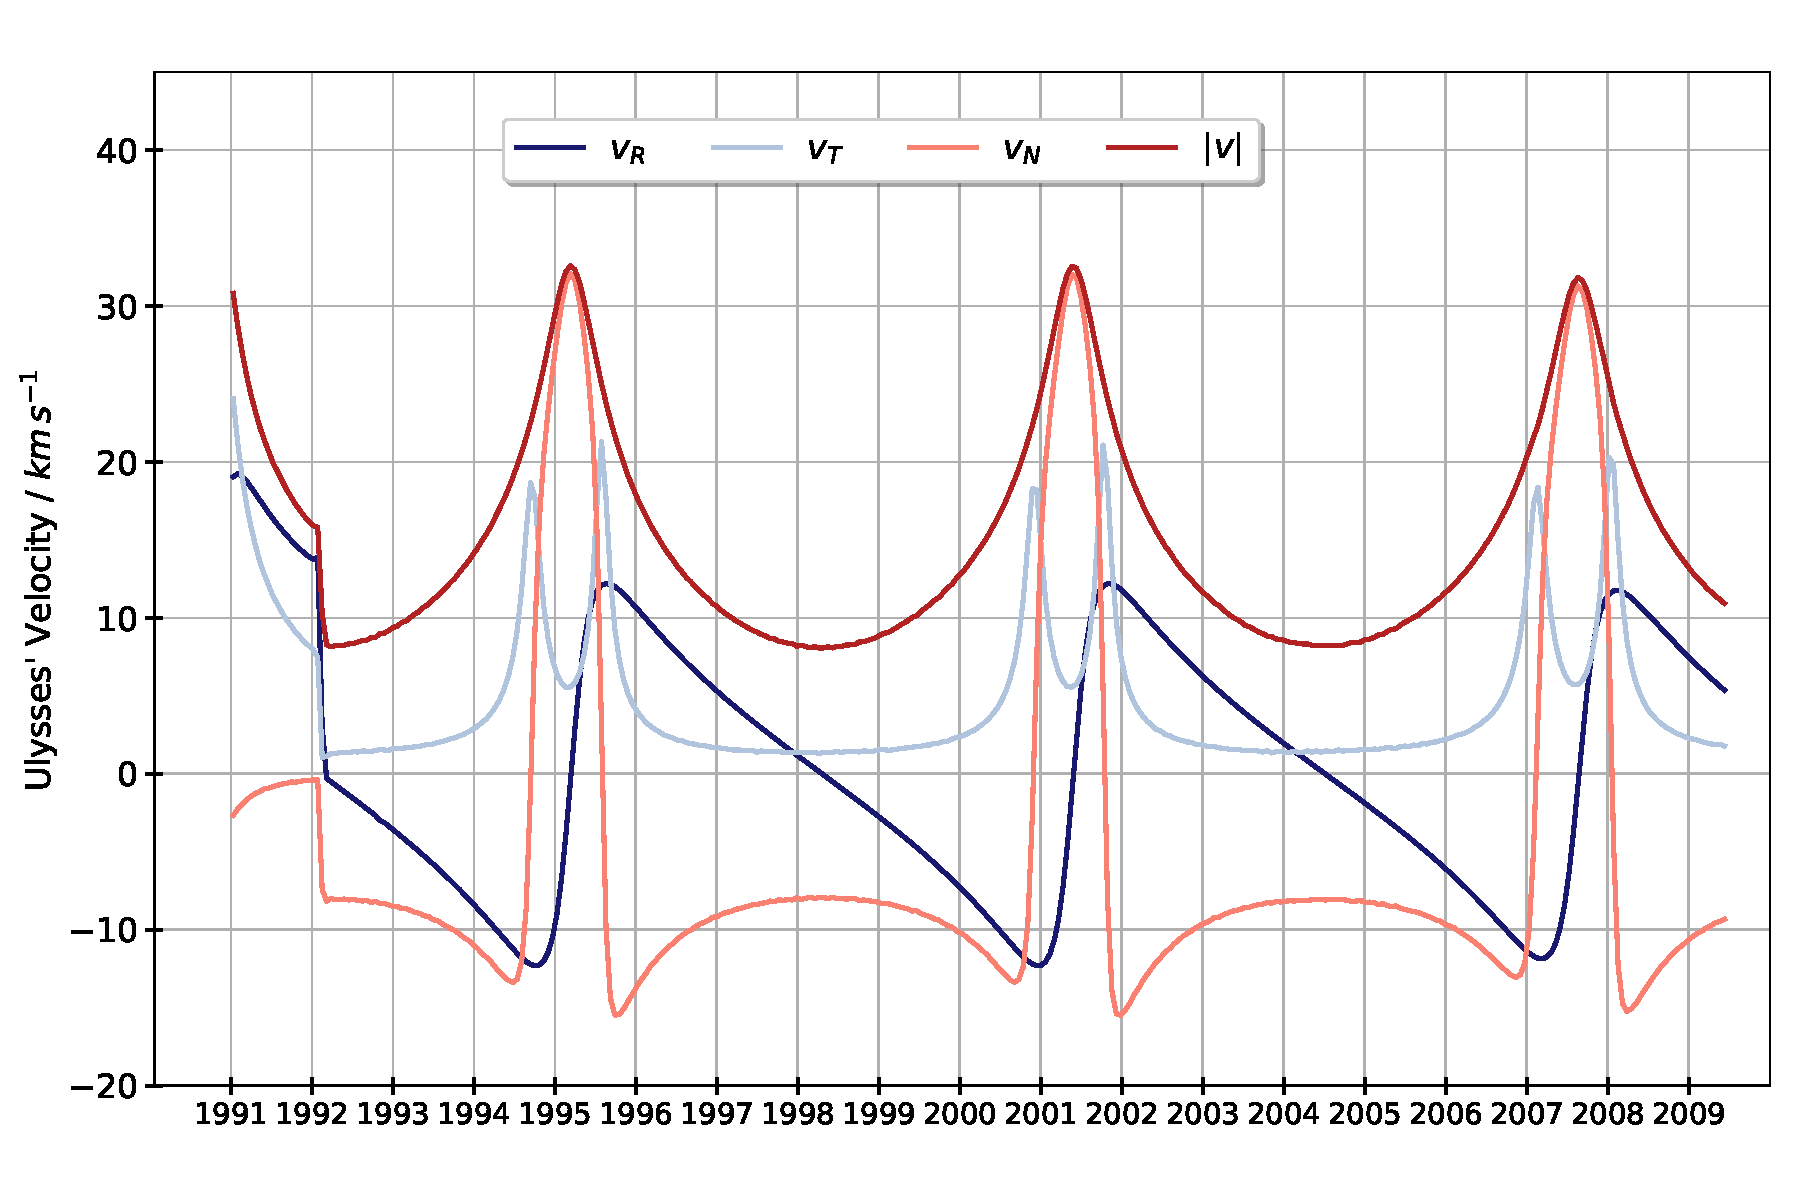
\includegraphics[width=1.\textwidth]{Figures/eigenv.pdf}
	\centering
	\caption{Eigen-velocity of Ulysses over the time of the mission. Shown are the RTN components and the absolute velocity.}
	\label{fig:eigenv}
\end{figure}




\subsection{Orientation of the Detector}
Until now we have assumed that Ulysses' spin axis is aligned with the R-axis of the coordinate system, i.e. that the spin axis points directly to the Sun. In fact, this is not the case in general. Due to telemetry reasons, Ulysses' high gain antenna has to be oriented directly towards Earth. As Ulysses' spin axis is aligned with the electrical axis of the antenna \citep{wenzel_ulysses}, it has an offset towards the spacecraft-Sun line. This offset is called aspect angle and is a permanently changing quantity as a function of Ulysses' position and the position of the Earth. Because a varying aspect angle results in SWICS covering different parts of velocity space it is essential to consider this quantity in detail.
%
%
\subsubsection{Calculation of the Aspect Angle}
The aspect angle is measured from the Ulysses--Sun line to the Ulysses--Earth line. To describe this angle uniquely for any moment, we need two spherical coordinates $\varphi_{\mathrm{asp}}$ and $\vartheta_{\mathrm{asp}}$ based on the RTN system. As shown in Fig.~\ref{fig:rtn}, $\varphi_{\mathrm{asp}}$ is measured in the $\vec{R}$--$\vec{T}$ plane between $-\vec{R}$ and the projection of the Ulysses--Earth line into this plane. $\varphi_{\mathrm{asp}}$  is $0^\circ$ for directions along $-\vec{R}$, that is the Ulysses--Sun line, and increases to positive values towards $-\vec{T}$. $\vartheta_{\mathrm{asp}}$ is the angle between the projection of the Ulysses--Earth line into the $\vec{R}$--$\vec{T}$ plane and the spin-axis. It is defined as $0^\circ$ for directions that lie within the $\vec{R}$--$\vec{T}$ plane and $+90^\circ$ for directions along $\vec{N}$.\\
For the calculation of the aspect angle we use the Ulysses trajectory data (s. Sec.~\ref{sec:cs}) and Earth trajectory data in heliographic coordinates on a daily basis from \citet{nasa-earth-coord} and converted both to RTN coordinates. In Fig.~\ref{fig:aa} both components $\varphi_{\mathrm{asp}}$ and $\vartheta_{\mathrm{asp}}$ as well as the ``flat'' aspect angle $\alpha$ with  $\alpha = \arccos(\cos{\varphi_{\mathrm{asp}}}) + \arccos(\cos{\vartheta_{\mathrm{asp}}}) -1$ are shown over the time of the mission. $\varphi_{\mathrm{asp}}$ varies in the range from $\sim - 25^\circ$ to $\sim 42^\circ$ and $\vartheta_{\mathrm{asp}}$ in a range from $\sim - 30^\circ$ to $\sim 17^\circ$. Large angles occur especially around the three fast latitude scans, i.e. when Ulysses is at its perihelion and has the smallest distance to Sun and Earth.
%%
%%
\begin{figure}[h]
	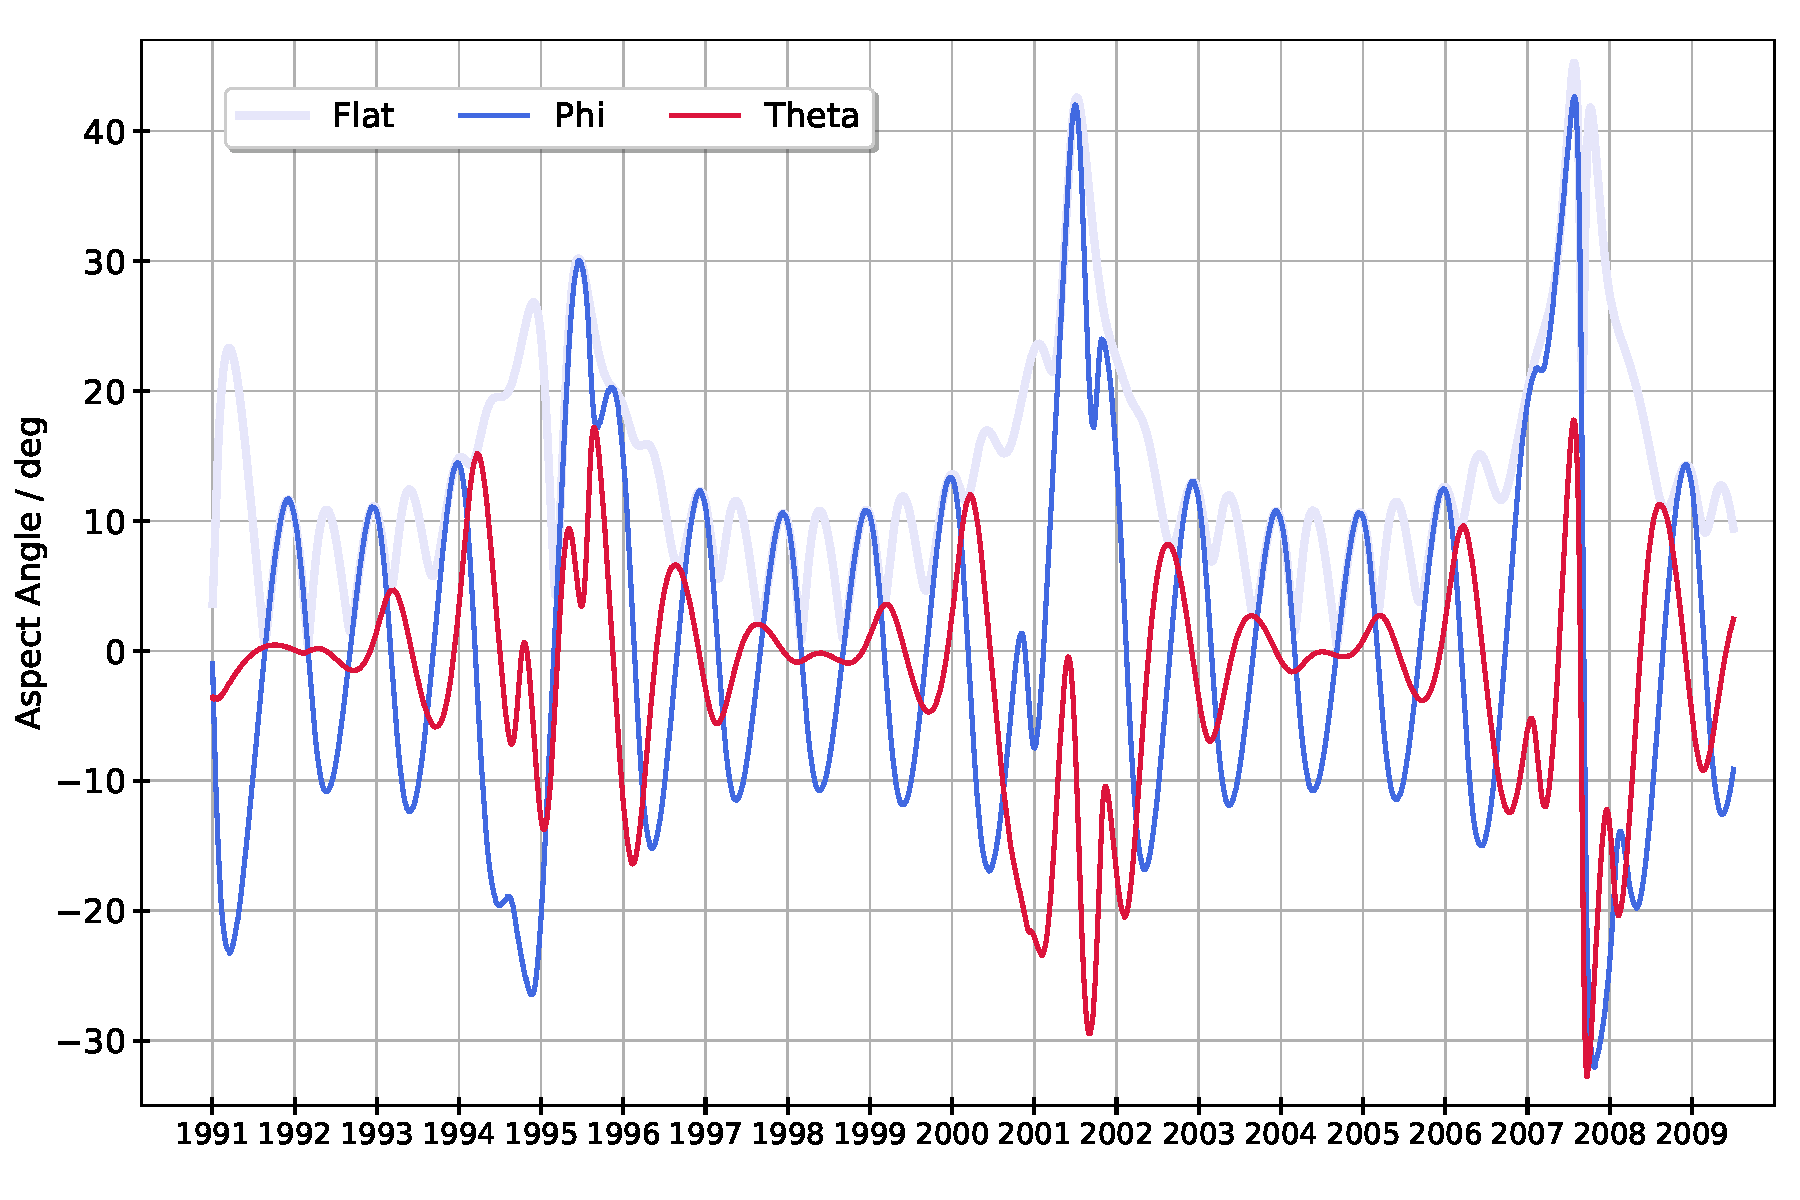
\includegraphics[width=1\textwidth]{Figures/aaa.pdf}
	\centering
	\caption{The evolution of Ulysses' aspect angle components $\varphi_{\mathrm{asp}}$ and $\vartheta_{\mathrm{asp}}$ and the ``flat'' aspect angle $\alpha$ with  $\alpha = \arccos(\cos{\varphi_{\mathrm{asp}}}) + \arccos(\cos{\vartheta_{\mathrm{asp}}}) -1$ from 1991 to the end of the mission. The aspect angle is the angle between the Ulysses--Sun line and the orientation of Ulysses' spin axis. A constantly changing aspect angle results from the fact that the spacecraft's antenna, which is nearly parallel to the spin-axis, has to point towards Earth all the time. Particularly large aspect angles occur during the three fast latitude scans around 1995, 2001 and 2007. Here, Ulysses' distance to Sun and Earth is at a minimum.}
	\label{fig:aa}
\end{figure}
\begin{figure}[h]
	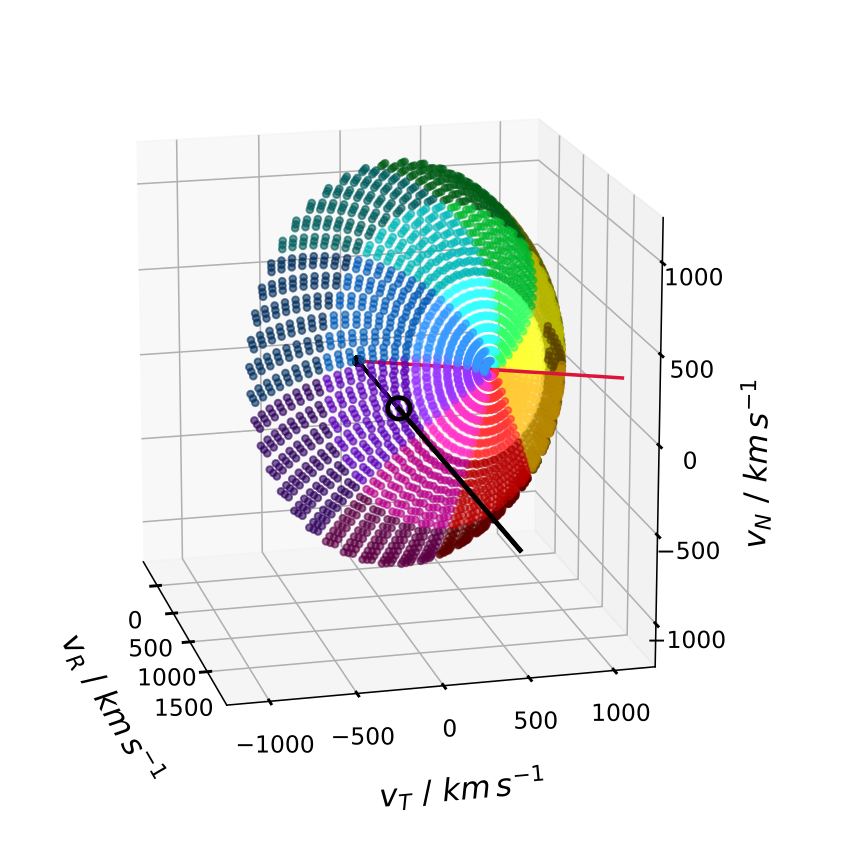
\includegraphics[width=0.7\textwidth]{Figures/col_aa_marker.png}
	\centering
	\caption{Velocity acceptance for ESA step 10 ($v \sim 1200 \,\mathrm{km\,s^{-1}}$) and for aspect angles $\varphi_\mathrm{asp} = 25^\circ$ and $\vartheta_{\mathrm{asp}} = -10^\circ $. Ulysses' spin axis is drawn in red and the radial direction in black. Marked is also the sector-detector element in  which an exclusively radial stream would be measured (black circle).}
	\label{fig:col_aa}
\end{figure}
%
%
%
The variable aspect angle is incorporated into the analysis by rotating the field of view corresponding to $\varphi_{\mathrm{asp}}$ and $\vartheta_{\mathrm{asp}}$. This results in a likewise rotation of the velocity acceptance space. In Fig. \ref{fig:col_aa} the acceptance velocity for the ESA step 10 ($v \sim 1200 \,\mathrm{km\,s^{-1}}$) is shown for $\varphi_\mathrm{asp} = 25^\circ$ and $\vartheta_{\mathrm{asp}} = -10^\circ $. Note that the orientation here seems to be mirrored with respect to the convention that has been described before. This is due to the inversion when transitioning from the field of view to velocity acceptance, s. Eq. \ref{eq:fov}.\\
When comparing Fig. \ref{fig:col_aa} with Fig.~\ref{fig:coll_FoV}, right panel, where a situation with $\vartheta_{\mathrm{asp}} = \varphi_{\mathrm{asp}} = 0$ is shown, it becomes clear that especially larger aspect angles change the link between a distinct sector-detector element and a volume in velocity space. While with a zero aspect angle a radial velocity (along $\vec{R}$) would be detected right in the middle of the velocity shell and definitely in the innermost detector, this is not the case for the aspect angle in Fig. \ref{fig:col_aa}. Here, an exclusively radially oriented velocity would be detected in a distinct sector in the central detector.\\
This also means that we can only transform a sector-detector measurement into a position in velocity space when we know about Ulysses' orientation!
\subsubsection{Consistency Check}
\label{sec:consis}
For checking if the considerations made before are reasonable and if the virtual detector works in the right way, we want to take a look at data of which we believe to know the velocity distribution function. Appropriate test data is the solar wind itself as it is believed to flow radially outwards from the Sun \citep[][,Ch. 6.1]{prlss_2004}. An ideal candidate within the solar wind is $\mathrm{He^{2+}}$ as the most abundant species. We can identify $\mathrm{He^{2+}}$ easily in Fig. \ref{fig:epq_rng0} and are provided with good statistics. Unlike protons, which are even more abundant in the solar wind, $\mathrm{He^{2+}}$ most likely deposits energy above the detector's threshold in the solid-state detector (s. Sec. \ref{subsec:det_eff}). This is because of its higher mass and the twice as high charge, which leads to a higher gain in energy by the post acceleration. Only when a particle triggers an $E_{\mathrm{SSD}}$ measurement (Triple Coincidence) we get a directional information about its velocity. Protons are most often measured as Double Coincidences except for suprathermal protons, for which the assumption of radial streaming must not hold true. For selecting $\mathrm{He^{2+}}$ we proceed like described in Sec. \ref{sec:etmatrices}.
\\ \\
In a first step we look at periods of time in which both aspect angle components $\varphi_{\mathrm{asp}}$ and $\vartheta_{\mathrm{asp}}$ are small ($<\pm5^\circ$). For these PHA words we draw a histogram of their sector and detector information. The result is shown in the left panel of Fig. \ref{fig:histdetsecaa}. The histogram shows that mainly the innermost detector is hit. This is the expected behavior when we imagine the instrument on a spacecraft that points directly to the Sun. A radially streaming flow then hits the instrument's detector that is oriented sunwards, which does not change with the spin of the spacecraft. This result is also consistent with the detector model for $\varphi_{\mathrm{asp}} = \vartheta_{\mathrm{asp}} = 0$ which is shown in Fig. \ref{fig:coll_FoV}. A radial stream can be represented here by the black line which cuts through the velocity shell in its center, the region of the innermost detector.
\\
In a second step we examine a time period in which Ulysses has a substantial aspect angle. This is particularly the case for when Ulysses is near its perihelion, s. Fig~\ref{fig:aa}. We choose for the second orbit, i.e. days 1-90 in 2001. For all $\mathrm{He^{2+}}$ PHA data from this time we again histogram sector and detector information, which is shown in the right panel of Fig. \ref{fig:histdetsecaa}. Compared to the left panel the maximum of counts is now shifted clearly towards a single sector, that is Sector No. 4, and to the central detector. This is consistent with the virtual detector in Fig. \ref{fig:col_aa}, where the aspect angle's value matches the measured one in the selected time period. Counts do not show up exclusively with this single sector-detector combination but slightly spread out over adjacent sector-detector elements. This is due to the fact that solar wind $\mathrm{He^{2+}}$ does not stream as an ideal beam but has a certain temperature, i.e. width \citep[][,Ch. 6.1]{prlss_2004}.


\begin{figure}
	\centering
	\begin{subfigure}{.5\textwidth}
		\centering
		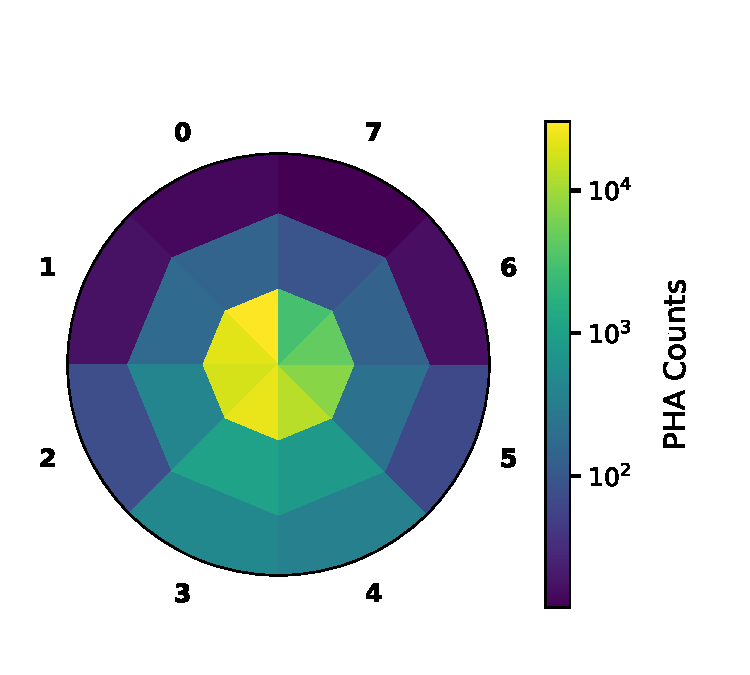
\includegraphics[width=1\textwidth]{Figures/hist_sec_det_noaa.pdf}
	\end{subfigure}%
	\begin{subfigure}{.5\textwidth}
		\centering
		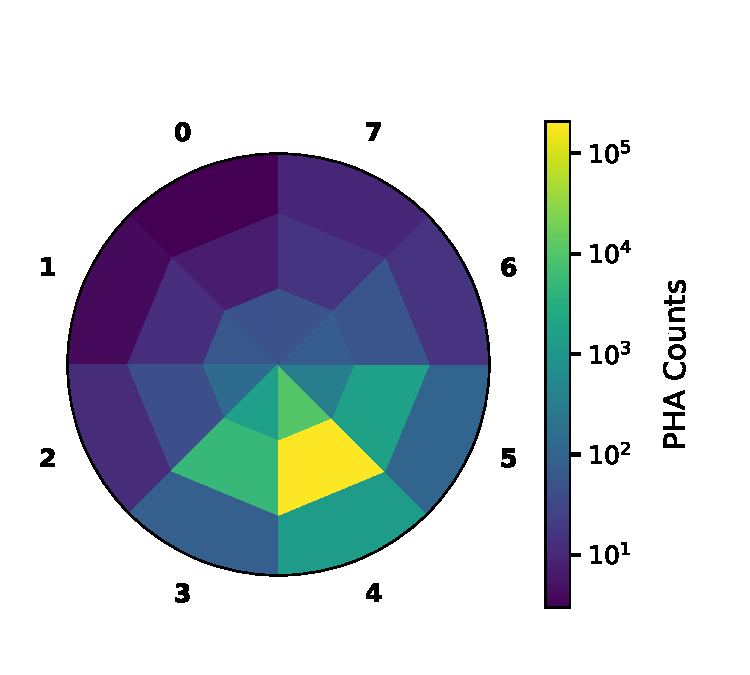
\includegraphics[width=1\textwidth]{Figures/hist_sec_det_aa.pdf}
	\end{subfigure}
	\caption{Histogrammed sector and detector information of $\mathrm{He^{2+}}$ PHA counts. \textbf{Left panel:} 365 days from 1992, $\varphi_{\mathrm{asp}}$ and $\vartheta_{\mathrm{asp}}$ limited to angles $<\pm5^\circ$. \textbf{Right panel:} DOY 1-90 from 2001  (large $\varphi_{\mathrm{asp}}$ and $\vartheta_{\mathrm{asp}}$).}
\label{fig:histdetsecaa}
\end{figure}
%
%
\subsubsection{Spin Reference Pulse}
In the previous section it was observed that $\mathrm{He^{2+}}$ PHA counts accumulate around the central detector for large aspect angles. Still it needs to be examined how the sectors are oriented.\\
As mentioned before, one spacecraft spin is divided into 8 sectors, starting with Sector 0 and ending with Sector 7. Every spin's start is defined newly by the ``spin reference pulse'' of Ulysses \citep{hiscale}. This pulse is triggered by a combination of four Sun sensors which detect when the Sun crosses a plane that is spanned by the spacecraft's spin axis and the spacecraft's x-axis, which is a particular axis perpendicular to the spin axis. The spin reference pulse is not uniform over time as the position of the Sun relative to the spacecraft changes with varying aspect angle.\\
To extract correct directional information from a sector data product of an ion that has been detected by SWICS it is essential to know the relative orientation between SWICS' main axis and the x-axis on the spacecraft. In the virtual detector this is implemented as an angle against the spacecraft--Sun line by which the field of view is rotated around the spin axis.\\
From the \citet[][p. 20-22]{swics_dpu} we know that the Sun pulse that triggers the beginning of Sector 0 is shifted by $180^\circ$ against SWICS' main axis. This means that the spacecraft has to rotate for a half spin after the Sun pulse until SWICS measures particles streaming radially from the Sun. However, it was possible to set a fine adjustment which would lead to an offset of the sun pulse from this center line up to $22.5^\circ$ \citet[][p.48]{swics_dpu}. Unfortunately, we do not know the value that has been chosen.
\\
If we assumed a wrong angle, a particle beam coming from a fixed direction in a Sun-fixed frame would be linked to a different direction. But this shift between true and supposedly measured direction is not constant over aspect angles. If we then measured over a longer time period with various aspect angles, we would measure the beam as blurred in velocity space.
\\
To make sure our model uses the right angle, we again choose $\mathrm{He^{2+}}$ as a test population of which we assume a beam-like behaviour streaming radially from the Sun. Also, we can only look at time periods when the aspect angles were large and the maximum of $\mathrm{He^{2+}}$ counts occurs in the central or outermost detector. Only here we can clearly discriminate between single sectors. When measured in the innermost detector the slightly widened distribution of $\mathrm{He^{2+}}$ would spread across all sectors as they are close together here.
From the right panel of Fig. \ref{fig:histdetsecaa}, where we histogrammed $\mathrm{He^{2+}}$ PHA words at a sizeable aspect angle, we find that the data is in agreement with the overall idea of a Sun pulse that is triggered a half spin before SWICS faces the Sun. If we believe the assumption that $\mathrm{He^{2+}}$ streams radially from the Sun, Sector 4, that is shifted by $180^\circ$ relative to Sector 0, contains the radial direction.\\ 
To check for a potential fine adjustment we search for tendencies of the maximum of counts sweeping to an adjacent sector. However, such a tendency that is consistent over time cannot be found. Thus, we proceed the analysis with the assumption that no significant fine adjustment had been set. 
%Zeigen: Für lange Zeiträume: $\mathrm{He^{2+}}$ kommt zentral. Für einzelne kurze: unterschiedlich.
%Deshalb: grober Check von wegen Detektor geht gut. Für das Feintuning (180 Grad oder doch was anderes?) reichts aber nicht...
\subsubsection{Transformation into $w$-space}
With the considerations of eigen-velocity and orientation of Ulysses we can use the virtual detector for translating $\mathrm{He^{+}}$ PHA words into the three-dimensional velocity space. Only when we have unfolded absolute velocities into their three components we can take the important step of transforming from a spacecraft frame of reference to a solar wind frame of reference. \\
Under the assumption that the solar wind streams basically radially this can be done by subtracting the instantaneous solar wind speed in R-component from a velocity in the spacecraft frame: 
\begin{align*}
\mathbf{v_{i,sw}} = \begin{bmatrix}v_{R,i,sc}\\v_{T,i,sc}\\v_{N,i,sc}\end{bmatrix} - \begin{bmatrix}v_{sw}\\0\\0\end{bmatrix}
\end{align*}
In a last step every component of the resulting vector is divided by the solar wind speed:
\begin{align*}
\mathbf{w_{i,sw}} = \begin{bmatrix}v_{R,i,sw} / v_{sw}\\v_{T,i,sw} / v_{sw}\\v_{N,i,sw} / v_{sw}\end{bmatrix}
\end{align*}
By this, the transition from a velocity space in the spacecraft frame to a solar wind independent $w$-space in the solar wind frame of reference is made.
%
%
%
%
\subsection{Velocity Space Coverage}
\label{subsec:cov}
When analyzing $\mathrm{He^{+}}$ PUI w-spectra with Ulysses SWICS, several effects have to be considered that limit the observable part of the w-space. The most obvious restriction results from the fixed geometry of the collimator (s. Sec. \ref{subsec:construction}), which allows to observe only a dome-shaped part of the $w$-space when considering the spin of the spacecraft and varying ESA steps.\\ (However, this dome is not fixed in $w$-space for different orientations of the spacecraft. While the ever changing aspect angle of Ulysses introduces a complex subject to directional data analysis it also enlarges the integrated coverage of velocity space over time.)\\
Furthermore, we have to deal with a limitation of the coverage in $w$ particularly for $\mathrm{He^{+}}$ triple coincidences. The observable range in ESA steps is 17 to 0, which for $\mathrm{He^{+}}$ corresponds to a limitation to velocities from $928\,\mathrm{km\,s^{-1}}$ to $1708\,\mathrm{km\,s^{-1}}$. While the upper limit is simply due to SWICS' highest possible ESA step, the lower limit is the lowest value for which $\mathrm{He^{+}}$ still has enough energy to overcome the threshold of the solid-state detector and thus can trigger a valid energy measurement (s. Sec.~\ref{subsec:det_eff}).\\
The $w$-range that is consequently covered is highly dependent on the prevalent solar wind speed. For $v_{sw} = 700 \,\mathrm{km\,s^{-1}}$ the absolute w in a spacecraft frame is limited to $1.2 < w_{SC} < 2.4$, whereas for slow solar wind at $v_{sw} = 300 \,\mathrm{km\,s^{-1}}$ the limitation is $2.9 < w_{SC} < 5.7$. 
In Fig. \ref{fig:cov} an exemplary w-space coverage for $v_{sw} = 700 \,\mathrm{km\,s^{-1}}$ and no aspect angle is sketched.\\
As we do not expect to measure the bulk of $\mathrm{He^{+}}$ at velocities $w_{SC}>>2$, we are thus limited to time periods with fast solar wind.
\begin{figure}[h]
	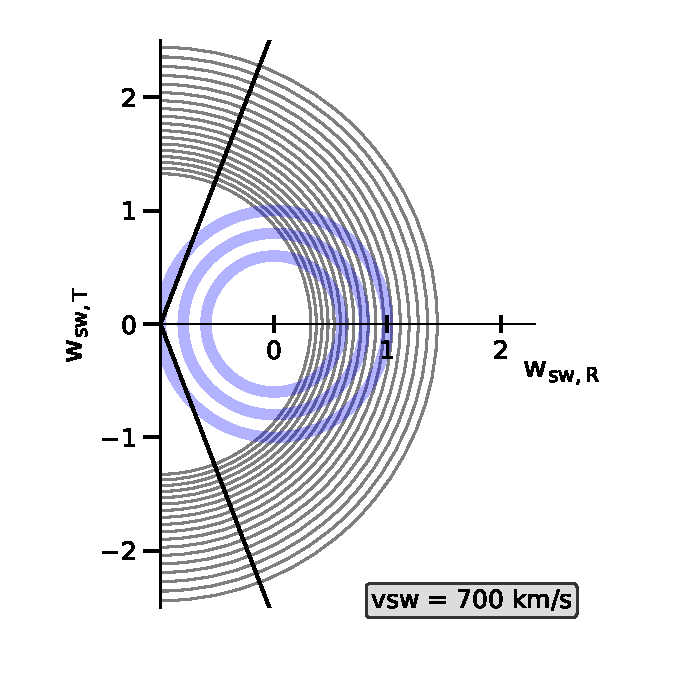
\includegraphics[width=0.8\textwidth]{Figures/covv.pdf}
	\centering
	\caption{SWICS' 2D projected $w$-coverage for $\mathrm{He^{+}}$ in the solar wind frame at solar wind speed $700\,\mathrm{km\,s^{-1}}$. Only ESA steps 0-17 are covered. The black lines is the coverage due to the detector geometry. Circles of constant $w$ in the solar wind frame are shown in blue for $w = 1$, $w = 0.8$ and $w = 0.6$.}
	\label{fig:cov}
\end{figure}
\\
In this work solar wind speed data is used that has been measured by the instrument SWOOPS \citep[Solar Wind Observations Over the Poles of the Sun,][]{bame_swoops} on Ulysses. \\ 
In Fig. \ref{fig:vsw_years} a histogram for occurring solar wind speeds is shown -- limited to times in which at least one $\mathrm{He^{+}}$ Triple Coincidences PHA event has been transmitted. The number on the right indicates the total number of $\mathrm{He^{+}}$ PHA triple coincidence data that was received within the year. One can see the overall variation of the solar wind speed that is due to different latitudes of the spacecraft: When close to the poles of the Sun, Ulysses is exposed to the fast solar wind \citep{mccomas_2004}, which is the case for example in 1995. Also, the total number of received data decreases heavily towards years in which Ulysses approaches the orbit's aphelion, e.g. 1998 at the end of the first orbit. This is mainly an effect of pickup ion flux reduction that scales with $r_\odot^{-2}$ due to the expansion of the solar wind \citep[][Ch. 6.1]{prlss_2004}.
\begin{figure}[h]
	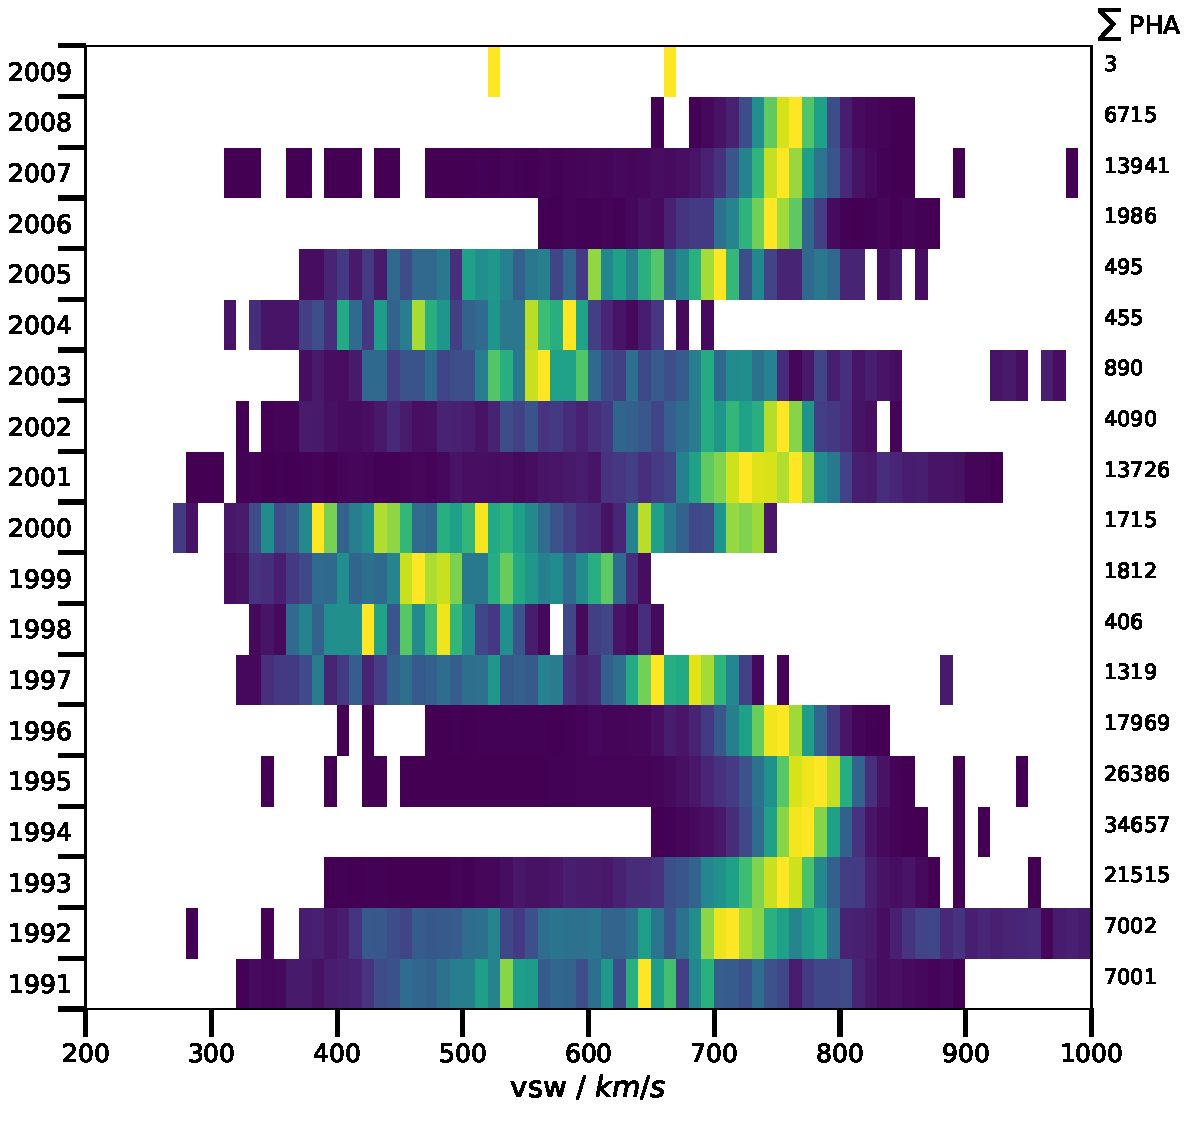
\includegraphics[width=1\textwidth]{Figures/vsw_sum.pdf}
	\centering
	\caption{Histogram of solar wind speed measured by SWOOPS for times in which $\mathrm{He^{+}}$ PHA data is measured by SWICS, sorted by years of the Ulysses mission. The color code is normalized to each year's maximum value (in yellow). In the right column one can find the total number of $\mathrm{He^{+}}$ PHA words per year. }
	\label{fig:vsw_years}
\end{figure}


%
\subsection{Phase Space Normalization}
We are now able to combine the information about sector, detector and ESA step from the selected $\mathrm{He^{+}}$ PHA triple coincidences with the information about how the spacecraft was moving and which direction it was facing at the time of the measurement.
Counts that we have collected over a certain time period can be mapped into three-dimensional w-space by this. However, for deriving physical quantities from these, a transition from counts to phase space density has to be performed.\\ \\
Firstly, we consider a single spin of the spacecraft, which normally corresponds to one ESA step of SWICS.
Counts $N_{jk}$ that have been measured in a phase space volume that has been covered by a sector-detector element $j$ during the ESA step $k$ can be connected to the average phase space density $\delta_{jk}$ in this volume by an integration over the three-dimensional velocity space:
\begin{align*}
N_{jk} &= \iiint\displaylimits_{v_{\varphi j}v_{\vartheta j}v_{R k}} \rho_{jk}	V_k	\,\,	d^3v,
\end{align*}
where $V_k = G \, \tau \, v_k$ is the spatial volume of the measurement with the geometrical factor $G = 0.0225 \,\mathrm{cm^2}$ (Dr. Lars Berger, personal communication), $\tau = 12/8\,\mathrm{s} = 1.5\,\mathrm{s}$ the time of the measurement in a single sector and $v_k$ the central velocity for $\mathrm{He^{+}}$ in the ESA step $k$.
With the opening angles of a single sector-detector element of $4^\circ$ in width and $69^\circ /3 = 23^\circ$ in length and the height of this element $\Delta v_k$ we can write
\begin{align*}
%&= \iiint\displaylimits_{v_{\varphi i}v_{\vartheta j}v_{R k}} \rho_{ijk} \,	G \, v_k \, \tau	\,\,	d^3v \\
N_{jk} &= v^2_k \left(\frac{\pi^2}{180^2}\cdot4 \cdot 23\right) \, \Delta v_k \, \rho_{jk} \,	G \, v_k \, \tau.
\end{align*}
$\Delta v_k$ is determined by the uncertainty in energy-per-charge measurements. It has been found to be $\Delta v_k = 0.025 \, v_k$ in Sec. \ref{subsec:construction}, which gives us
\begin{align*}
N_{jk} &= v^4_k \left(\frac{\pi^2}{180^2}\cdot4 \cdot 23\right) \, 0.025\, \rho_{jk} \, G  \, \tau.
\end{align*}
This can be rewritten as an expression for the average phase space density $\delta_{jk}$ with the phase space volume $V_{k}$ as 
\begin{align*}
\rho_{jk} &= \frac{N_{jk}}{V_{k}}.
\end{align*}
Note that $V_{k}$ is only dependent on the ESA step $k$, as the sector-detector elements span the same (absolute) phase space volume for one step.\\
When we want to measure more than one spin, we need to consider that the probability to detect an ion is dependent on the ESA step. This behavior is described in Sec. \ref{subsec:det_eff} as the detection efficiency.\\
For phase space normalization this is considered by weighting the spanned phase space volume for every sector-detector element with the efficiency of the respective ESA step $\mathrm{eff}_k$: 
\begin{align*}
\rho_{jk} &= \frac{N_{jk}}{V_{k}\cdot \mathrm{eff}_k}
\end{align*}
To consider the resolution of the single sector-detector-ESA elements (s. Sec. \ref{subsec:construction}) we assign each of the velocity acceptances in an element the count rate $\frac{1}{n_i}\, N_{jk}$ and the partial phase space volume $\frac{1}{n_i} \, V_{k}$.\\
As we will not always have counts in every scanned phase space volume, we have to integrate over longer periods of time to determine a phase space density.
As the instrument covers different phase space volumes with varying aspect angle, changing parts of phase space volume are covered. To take this into account we have to divide the integrated count rate in a distinct volume by the integrated volume over all time in which this volume has been observed -- independent on whether a PHA event has been measured.
%.
%\\ \\ \\
%Mittlere Phasenraumdichte in einem Bin, in den zwei Instrumentenbins A und B reingehen:
%(differential PSD)
%\begin{align}
%\bar{\rho} = \frac{N_A + N_B}{\frac{N_A}{N_{A,ges}} V_A + \frac{N_B}{N_{B,ges}} V_B }
%\end{align}
%Dabei ist $N_i$ die Anzahl der Hits, die im Messbin gelandet sind und $N_{i,ges}$ die gesamte Anzahl an Bins. Hits heißt GEsamtcounts durch Detektoranzahl. Eigentlich gebe ich statt $N_i$ $N_i \cdot Detektoranzahl$ rein, aber das kürzt sich ja raus.\\ \\
%Effizienz und Sektorgewichte dazu:\\
%Allg.:
%\begin{align*}
%\rho = \frac{N \cdot brw}{V \cdot Eff}
%\end{align*}
%Und dann
%\begin{align}
%\bar{\rho} = \frac{N_A + N_B}{\frac{N_A}{N_{A,ges}} \frac{V_A \cdot eff_A}{brw_A} + \frac{N_B}{N_{B,ges}} \frac{V_B \cdot eff_B}{brw_B} }
%\end{align}








